% Created 2016-08-12 Fri 19:20
\documentclass{article}
\usepackage[utf8]{inputenc}
\usepackage[T1]{fontenc}
\usepackage{fixltx2e}
\usepackage{graphicx}
\usepackage{longtable}
\usepackage{float}
\usepackage{wrapfig}
\usepackage{rotating}
\usepackage[normalem]{ulem}
\usepackage{amsmath}
\usepackage{textcomp}
\usepackage{marvosym}
\usepackage{wasysym}
\usepackage{amssymb}
\usepackage{hyperref}
\tolerance=1000
\usepackage{minted}
\usepackage{listingsutf8}
\usepackage{enumitem}  %% for lists (in algorithm)
\usepackage{mathtools} %% for \coloneqq
\usepackage[bottom]{footmisc} %% to keep entire footers on one page
\usepackage[]{graphicx}
\usepackage[]{minted} %% for code snippets
\usepackage[a4paper,margin=1in]{geometry}
\usepackage{comment}
\usepackage[linesnumbered,ruled,lined,shortend]{algorithm2e}
\usepackage[space]{grffile}
\setcounter{secnumdepth}{4}
\author{Nicholas Mitchell}
\date{\today}
\title{4\_Gradient\_Boosting}
\hypersetup{
  pdfkeywords={},
  pdfsubject={},
  pdfcreator={Emacs 24.5.1 (Org mode 8.2.10)}}
\begin{document}

\maketitle
\tableofcontents

\pagebreak

\section{Gradient Boosting \label{chapter-gradient-boosting}}
\label{sec-1}


\subsection{What is boosting? \label{AdaBoost}}
\label{sec-1-1}

There were several important developments that were necessary to arrive at the model that this study ultimately uses. They are each addressed in the following sections, and may be summarised as follows:

\begin{enumerate}
\item The first \textbf{boosting} algorithm was defined: AdaBoost \cite{freund1996experiments}, \cite{Freund1997119}
\item AdaBoost was re-formulated as \textbf{gradient descent}, taking a special loss function \cite{Breiman97arcingthe}, \cite{breiman1998arcing}
\item AdaBoost was generalised to allow a multiplicity of loss functions: \textbf{gradient boosting} \cite{friedman2001greedy}, \cite{friedman2000additive}
\end{enumerate}

The generalised final product, gradient boosting, can be used for regression, classification and ranking problems, making it a tool with a diverse range of applications, in many different contexts.

As listed above, the first notions of boosting stem from work by Freund and Schapire, in which they developed an algorithm named \emph{AdaBoost} (full form: adaptive boosting\footnote{A qualitative description only is given here. For a more detailed illustration, please refer to the referenced literature.}) that gradually improves model performance on a given data set over a number of iterations. Instead of defining one complex function, AdaBoost iteratively fits a simple model - a \emph{base-learner} - to the data set. Before the first iteration, all data points are considered of equal importance, and so uniformly weighted. In the case of regression with square loss, the residual errors produced from each iteration (labelled the \emph{shortcomings}) are subsequently used to re-weight the data points. Each falsely classified point receives more weight (proportional to the log-odds of the previous iteration's weighted error) and, in a similar fashion, the weights of the correctly classified data points are decreased. Finally, all weights are normalised to sum to unity before the next iteration\footnote{As each step is reliant on the previous, the models that are fitted are not independent from one another. Within the context of machine learning, this is often termed an \emph{ensemble method}.}. This weight adjustment steps instructs the naive model how to prioritise its fit or classification in the following iteration - targeting areas where the model performs weakly. It is possible that many mistakes are made by the naive base-learner used at each stage throughout the process; however, the weights reflect how many times each point was classified falsely, and it is the sum of these weights that defines the final model.

The shortcomings are the residuals from each fit, which are used to iteratively re-fit a function. The model is updated after each iteration of re-modelling on the shortcomings, thus incrementally improving the model and decreasing the observed error on the data set. If this overall error is thought of as a function of the model to be minimised, then the residuals correspond to the negative gradient of that function. In order to generalise the AdaBoost methodology for other loss functions, (as is described in the following sections), it is more useful to retain this concept of gradients when referring to the shortcomings of a model. Re-expressing the boosting methodology of AdaBoost in this generalised way: we are making approximations to the gradient of a loss function in each step - this leads to the descriptive name \emph{functional gradient descent} (FGD).


\subsection{Building on the basics \label{linear-model}}
\label{sec-1-2}

The simple idea of linear regression (\cite{hyndman2014forecasting} ch.4) may be thought of as the fundamental idea behind much of the boosting methodology used in this study. It is what is often used as a starting point\footnote{Here we mean in terms of a base-learner and initial \emph{go-to method} before more complicated models are considered.} when building a boosting-based model and so may be considered an elementary building block e.g. when defining in a generalised linear model (GLM).

We consider a function, $f : \mathbf{X} \rightarrow \mathbf{Y}$, that describes a data set by mapping an input, $\mathbf{X} = \left\{ X_1, X_2, … , X_n \right\}$, to a response variable $\mathbf{Y}$. Given the input and output variables, it is this function, which is to be approximated. In the classic example of linear regression, this means placing a straight line over or through the data set, which is as close as possible to as many of the points within that data set as possible. The \emph{goodness of fit} of that line can be quantified and so assessed by some metric on the distance found between the line and each of the individual points. In the case of the ordinary least squares (OLS) methodology\footnote{If errors are assumed to be normally distributed, we could instead refer to the \href{https://en.wikipedia.org/wiki/Maximum_likelihood}{maximum likelihood estimation (MLE)$^{\dag{}}$}.}, this is achieved by summing the \emph{squares} of the distances between each point and the line, and then adjusting the line so that defined sum becomes as small as possible; thus the problem is one of minimisation\footnote{More generally speaking the problem is one of optimisation; minimisation when optimising over a loss function, however \emph{maximisation} when optimising over a likelihood function}. To help visualise this, the distances are highlighted by red arrows in Figure \ref{fig:basic.residuals}, which is a short excerpt of some sentiment analysis data (see Section \texttt{data-exploration} for more information regarding the data used in this study). It is the sum of these lengths squared that is to be minimised by moving the line. We notice that the lines are all vertical, which is because we are interested only in the distance (also called the error or the residual) between the outcome variable that our line would predict for a given input value on the x-axis, and the \emph{true} outcome, i.e. the y-coordinate of the corresponding point from the data set.

\begin{figure}[htb]
\centering
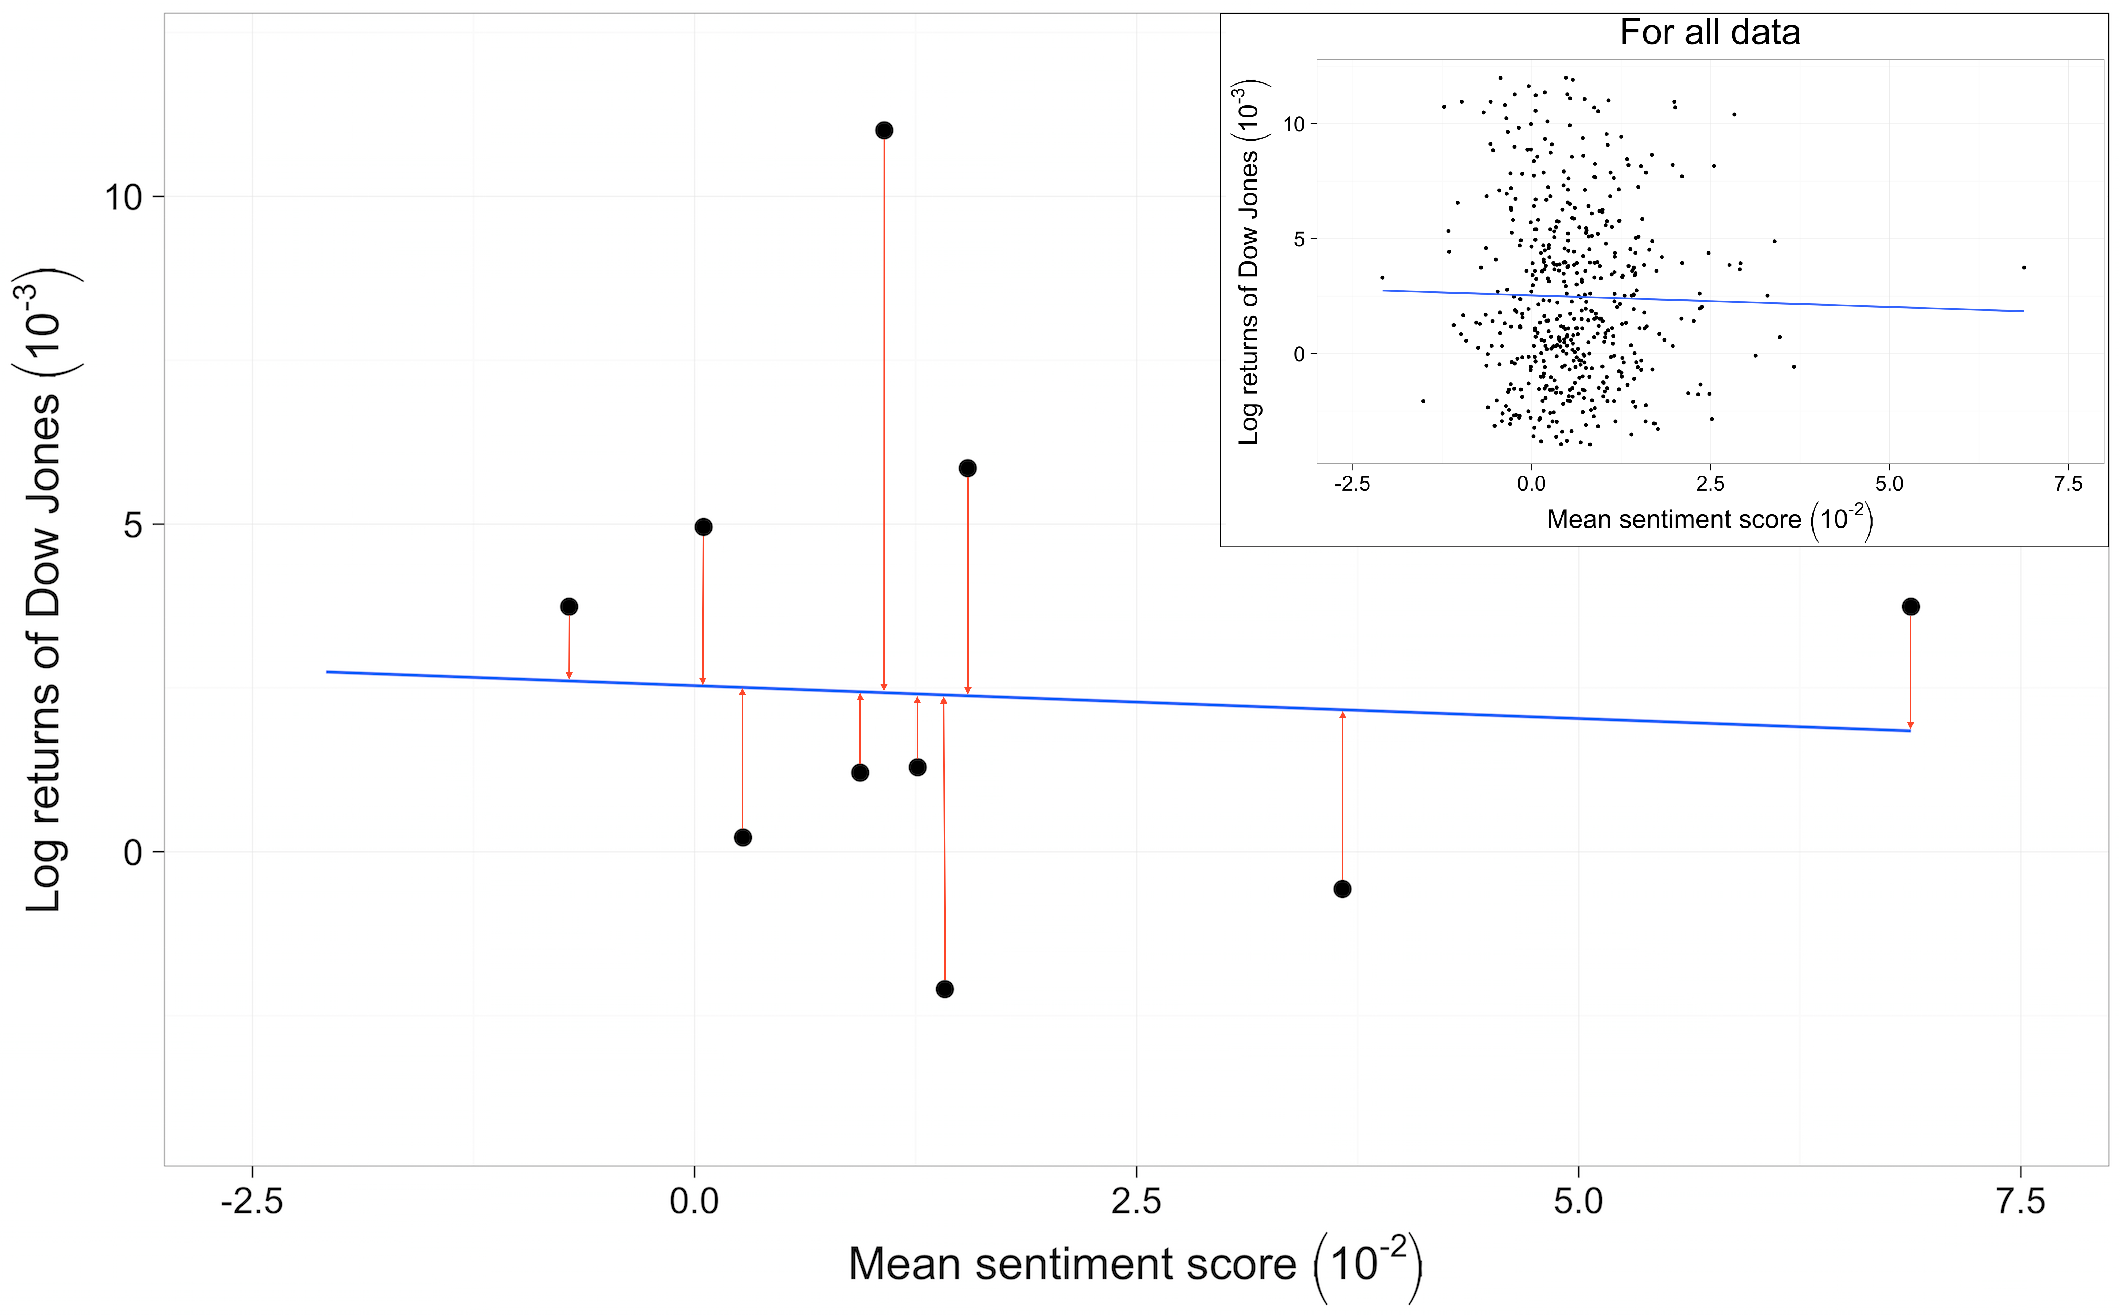
\includegraphics[width=16cm]{/Volumes/Mac OS Drive/Thesis/Source Code/Reporting/nwm_Report/images/basic_residuals.png}
\caption[An example of linear regression using sentiment analysis scores]{\label{fig:basic.residuals}Sentiment scores of term "dow jones" versus Dow Jones returns of following day. Ten consecutive days are randomly selected and displayed with their residual errors as red arrows to the regression line, which is produced via a linear fit over all 695 data points. Inset: the same plot without error highlighting, including all data points.}
\end{figure}

The line represents our function, an approximation to the data set, and describes a one-dimensional response variable $Y$ with one explanatory variable $X$. As will be shown in the following sections, this is often the case in component-wise gradient boosting, where a single variable vector is regressed on the single response variable (or iteratively on the residuals of consecutive fits).


\subsection{Gradient boosting \label{grad-boosting}}
\label{sec-1-3}


\subsubsection{The objective \label{basic-problem}}
\label{sec-1-3-1}

The goal of gradient boosting is the same as any other (in this case, forecasting) model: to fit a function to a data set that accurately describes the data and allows for new input data points to make predictions on the outcome variable, all while minimising error. Consider a sample containing $n$ values for each of $p$ predictor variables $\mathbf{X = (X_1, X_2, … , X_p)^\top}$, along with a corresponding one-dimensional\footnote{Vector notation is used here, where $\mathbf{X_1}$ represents the vector $(X_1, X_2, … , X_n)$ for $p = 1$.} \emph{outcome variable}: $\mathbf{Y}$. The goal is then to find the optimal function $f^* (\mathbf{X})$ that describes the given data and allows predictions to be made for $\mathbf{Y}$. The method should not be a \emph{black-box} \footnote{Neural networks are the standard example of such a model. High predictive accuracy may be obtained, but the modelling process does not allow for much interpretability. The characteristic of the final model being \emph{non-identifiable} increases difficulty of further analysis. \href{http://colah.github.io/posts/2014-03-NN-Manifolds-Topology/}{Recent advancements with visualisations$^{\dag{}}$} into the understanding of the \emph{hidden layers} have, however, been made.}, i.e. it must be transparent at all stages, and the final model $f^*$ should permit the interpretation of results and interactions between features.

A classic (simple) approach might fit additive regression models using MLE, such as the the linear model example described in Section \texttt{linear-model,} applied to each predictor individually. The output of such a model would then take the form shown in Equation \eqref{eqn-additive-model}, which has the structure of an additive predictor provided by a general additive model (GAM) \cite{Hastie2009} and the functions $\hat f_{1} + … + \hat f_{p}$ each correspond to the linear functions (later defined as the base-learners). These functions depend only on the predictor variables that were used as inputs. We shall see that single variables are generally use as inputs for each base-learner; however, subsets of variables may be allocated to each base-learner.

\begin{equation}
  \label{eqn-additive-model}
  f^* (\mathbf{X}) = \beta_0 + f_1 (\mathbf{X_1}) + f_2 (\mathbf{X_2}) + … + f_p (\mathbf{X_p})
\end{equation}

\vspace{3mm}

There are several points to consider when using such a model, i.e. when selecting base-learners and the subsets of variables to be used as input. Two examples, both of which indeed present themselves in this study's data set, are (1) high levels of pairwise-correlation between predictors, and (2) cases in which we have \emph{wide} data sets ($p > n$). The questions that arise, regard matters such as the explanatory power attainable in the face of $m$ highly correlated variables being included in one model, and then which of those variables provides the most information. A model that can cope with such input data should ideally include an \emph{in-built} method of variable selection that can deal with multicollinearity, and also may return a sparse model, i.e. not all predictors must be included in the final model. Gradient boosting provides a framework in which those concerns are addressed satisfactorily, particularly because each step of the modelling procedure is transparent, allowing errors in modelling assumptions to be identified.

The naive approach to variable selection by means of exhaustively fitting models for all possible subsets of predictors is not an option when the data sets are wide, i.e. with large $p$. More systematic methods of variable selection, especially the case of wide data sets, can be difficult to perform and do not guarantee the optimal solution. Examples of step-wise search techniques include \emph{backward} and \emph{forward selection}, which avoid exhaustive model fitting. While reducing the number of models fitted, these methods cannot guarantee optimality as the explanatory power of feature interactions is not necessarily considered (most easily demonstrated with forward selection - \cite{Fukunaga1990441} ch.10).


\subsubsection{General properties \label{gen-props}}
\label{sec-1-3-2}

Gradient boosting provides a \emph{fitting method} that minimises an empirical risk (loss) function\footnote{Empirical risk and loss function are used synonymously. Depending on the context, other names are also given to the same principle, for example: a cost function (neural networks) and the hinge loss (support vector machines), to name just a few.} with respect to a given prediction function $f$. The risk function component is modular, meaning it may take many forms, in each case describing a particular loss function, which is to be minimised\footnote{This terminology is commonly used in \href{https://en.wikipedia.org/wiki/Data_mining}{\emph{data mining$^{\dag{}}$}} communities; however, the distinction between minimising \emph{loss functions} in data mining and maximising \emph{likelihood functions} in classical statistics is rather hazy.}. Examples are the $L_1$ (Laplace), $L_2$ (Gaussian), Huber, exponential and negative log-likelihood loss functions\footnote{For more detail on unbiased estimators that minimise a risk, refer to Ch. 3 of \cite{pfanzagl1994parametric}}. In order to minimise such functions, they must be convex and continuously differentiable so that the first derivative may be solved over any interval. There are particular applications of loss function minimisation that make the even stronger assumption that the loss-function be Lipschitz continuous \cite{dimitrakakis2013differential}, which places an upper bound on the magnitude of the gradient of the function over an interval. Two exceptions to continuous differentiability are the $L_1$ and hinge loss functions, which are non-differentiable at their inflection points. In software implementations this discontinuity is often set to zero as to prevent a computational error being thrown (the gradient being undefined at the inflection points), thus allowing stable usage\footnote{The $L_1$ loss function has been shown, theoretically as well as experimentally, to achieve superior performance to the alternatives in certain cases - especially in \emph{sparse} models, where few coefficients are found to be non-zero (see \cite{Hastie2009} p.611-613)}.
The results of boosting are generally in the form of an \emph{additive} predictive function, as depicted by Equation \eqref{eqn-additive-model}, and so are readily interpreted. The further benefits that are reaped by using component-wise gradient boosting\footnote{Component-wise gradient boosting is specifically addressed in Section \ref{comp-boosting}.} will become apparent as the methodology is explored in the following sections, but may first be summarised here by stating that component-wise boosting:

\begin{enumerate}
\item is applicable for use with a wide range of loss functions (as described above),
\item is able to perform variable selection during the fitting process,
\item can perform well in situations where $p>>n$, e.g. genetics
\item inherently addresses multicollinearity between predictors, shrinking effect estimates towards zero,
\item optimises prediction accuracy with respect to a given risk function, and
\item offers high transparency throughout the modelling iterations.
\end{enumerate}


\subsubsection{Naive functional gradient descent \label{naive-boosting}}
\label{sec-1-3-3}

We first define the basic approach to gradient boosting, describing how gradient descent is performed. At the same time, specific applications are introduced within the context of this study. The component-wise version that was ultimately used is presented in the sections that follow.
We start with the initial model, slightly extending that given in Section \ref{basic-problem}, by again considering a one-dimensional response variable $\mathbf{Y}$, but with a $p$-dimensional set of predictors $\mathbf{X = (X_1, X_2, … , X_p)^\top}$. A model that aims to fit a model that explains this relationship may be presented thusly:

\begin{equation}
  f^* \coloneqq \underset{f(\cdot)}{argmin{\ \mathbb{E}_{\mathbf{Y,X}}}}[\rho (\mathbf{Y}, f(\mathbf{X}))]
      \label{eqn-optimise}
\end{equation}

\vspace{3mm}

where $\rho$ is a loss function with the properties described in Section \ref{gen-props}. The optimal model $\hat f(\cdot) = f^*$ therefore minimises the expected loss, i.e. the error. This study looks at several loss functions\footnote{The Gaussian $L_2$ loss function is used in Section \texttt{results-gauss}.} that are able to be inserted into Equation \eqref{eqn-optimise}; two examples of which are the \emph{absolute loss} - illustrated in Equation \eqref{eqn-bin-loss} - and the \emph{squared loss} (used in Gaussian regression) - illustrated in Equation \eqref{eqn-gauss-loss}.

%% Binomial
  \begin{equation}
    \underset{\ell{_1}}{\rho} = |\mathbf{Y} - f(\mathbf{X})|
    \label{eqn-bin-loss}
  \end{equation}

%% Gaussian
  \begin{equation}
     \underset{\ell{_2}}{\rho} = (\mathbf{Y} - f(\mathbf{X}))^2
    \label{eqn-gauss-loss}
  \end{equation}

\vspace{3mm}

Modelling is performed on a sample set with $n$ realisations $X = (X_1, X_2, … , X_n)$ and $Y = (Y_1, Y_2, … , Y_n)$ of $\mathbf{X}$ and $\mathbf{Y}$, respectively, and so an exact expectation for Equation \eqref{eqn-optimise} is unknown. Instead, boosting algorithms minimise an empirical risk function (the \emph{observed mean}) with respect to some approximation function, $f(\cdot)$, given as:

%% General empirical risk
\begin{equation}
  \label{eqn-emp-risk}
  \mathcal{R} = \frac{1}{n} \sum_{i=1}^{n} \rho(Y_i, f(X_i))
\end{equation}

\vspace{3mm}

Referring once again to the principle of modularity, either of the two loss functions given in Equations \eqref{eqn-bin-loss} and \eqref{eqn-gauss-loss} (plus \emph{any} other defined loss functions that fulfils the requirement of convexity and continuous differentiability) may be inserted into the empirical risk function given by Equation \eqref{eqn-emp-risk}. Equation \eqref{eqn-gauss-emp-risk} shows the case for the $L_2$ loss function.

%% Gaussian empirical risk
\begin{equation}
  \mathcal{R} = \frac{1}{n} \sum_{i=1}^{n} (Y_i - f(X_i))^2
  \label{eqn-gauss-emp-risk}
\end{equation}

\vspace{3mm}

The next step is to establish the iterative \emph{gradient descent} method, which minimises $\mathcal{R} = \mathcal{R}(f_{(1)}, f_{(2)}, … , f_{(n)})$ with respect to the approximation function, $f_{(\cdot)}$; where $f_{(1)} = f(X_1), f_{(2)} = f(X_2), … , f_{(n)} = f(X_n)$. We notice that these each are merely output numbers, meaning we can simply treat $f(X_i)$ as parameters and take derivatives with respect to Equation \eqref{eqn-emp-risk}, which for the case of an $L_2$ loss function, as in Equation \eqref{eqn-gauss-emp-risk}, yields:

\begin{equation}
  \label{eqn-loss-derivative}
  \frac{\partial \mathcal{R}}{\partial f(X_i)} = \frac{\partial}{\partial f(X_i)}\left(  \sum_{i=1}^{n} \rho(Y_i, f(X_i)) \right) = \frac{\partial}{\partial f(X_i)}\left(  \rho(Y_i, f(X_i)) \right) = f(X_i) - Y_i
\end{equation}

\vspace{3mm}

which illustrates the relationship between the residuals and the negative gradient of the cost function, thereby demonstrating the reason why the former may be interpreted, in a more general manner, via the latter. By simple re-arrangement:

\begin{equation}
  Y_i - f(X_i) = - \frac{\partial \mathcal{R}}{\partial f(X_i)}
  \label{eqn-residuals-loss}
\end{equation}

\vspace{3mm}

We define initial conditions by first setting the approximation functions $f_{(\cdot)}$ to some offset values $\hat f_{(1)}^{[0]}, … ,\hat f_{(n)}^{[0]}$, where an iteration counter $m$ is set to zero (shown in the superscript of $f_{(\cdot)}$). In each step, an approximate to the gradient of the loss function is computed and used to update the approximation functions as follows:

\begin{equation}
  \label{eqn-naive-increment}
  \left(  
    \begin{array}{c}
      \hat{f}_{(1)}^{[m]} \\           
      \vdots \\
      \hat{f}_{(n)}^{[m]}
    \end{array}
  \right) =
  \left(  
    \begin{array}{c}
      \hat{f}_{(1)}^{[m-1]} \\           
      \vdots \\
      \hat{f}_{(n)}^{[m-1]}
    \end{array} 
  \right) +
  \nu \cdot 
  \left(
    \begin{array}{c}
      - \frac{\partial}{\partial f_{(1)}}(\hat{f}_{(1)}^{[m-1]}) \\ 
      \vdots \\
      - \frac{\partial}{\partial f_{(n)}}(\hat{f}_{(n)}^{[m-1]})
    \end{array}
  \right)
\end{equation}

\vspace{3mm}

where $\nu$ is the learning rate, or \emph{step length factor} - see Section \ref{nu} for more discussion on this model parameter. With each iteration of the model, we notice the approximation functions (and so the coefficients), as shown in Equation \eqref{eqn-naive-increment}, are \textbf{all} simultaneously incremented\footnote{Because all values $f(X_i)$ are updated in each iteration, this procedure may be referred to as \emph{batch} gradient descent. This highlights the difference to \emph{component-wise} gradient descent, described in Section \ref{comp-boosting}.} in each iteration, by an amount proportional to the gradient of the loss function. This is explicitly analogous to the \emph{shortcomings} of AdaBoost (the residuals themselves) being used to improve the model (Section \ref{AdaBoost}) and embodies the principle of steepest descent: the coefficients take the shortest path to their final estimates that minimise the loss function. Because of this feature, the algorithm is also know as \emph{greedy} \cite{friedman2001greedy}, \cite{Hastie2009}. The process is illustrated in Figure \ref{fig:contour_plot}, which represents a contour plot of a fictitious cost function. The process is repeated until the algorithm converges to the values $\hat f_{(1)}^{[m_{stop}]} , … , \hat f_{(n)}^{[m_{stop}]}$, which correspond the best approximation to the loss function's minimum. Here, m$_{\text{stop}}$ represents the number of iterations required to reach this minimum.

\begin{figure}[htb]
\centering
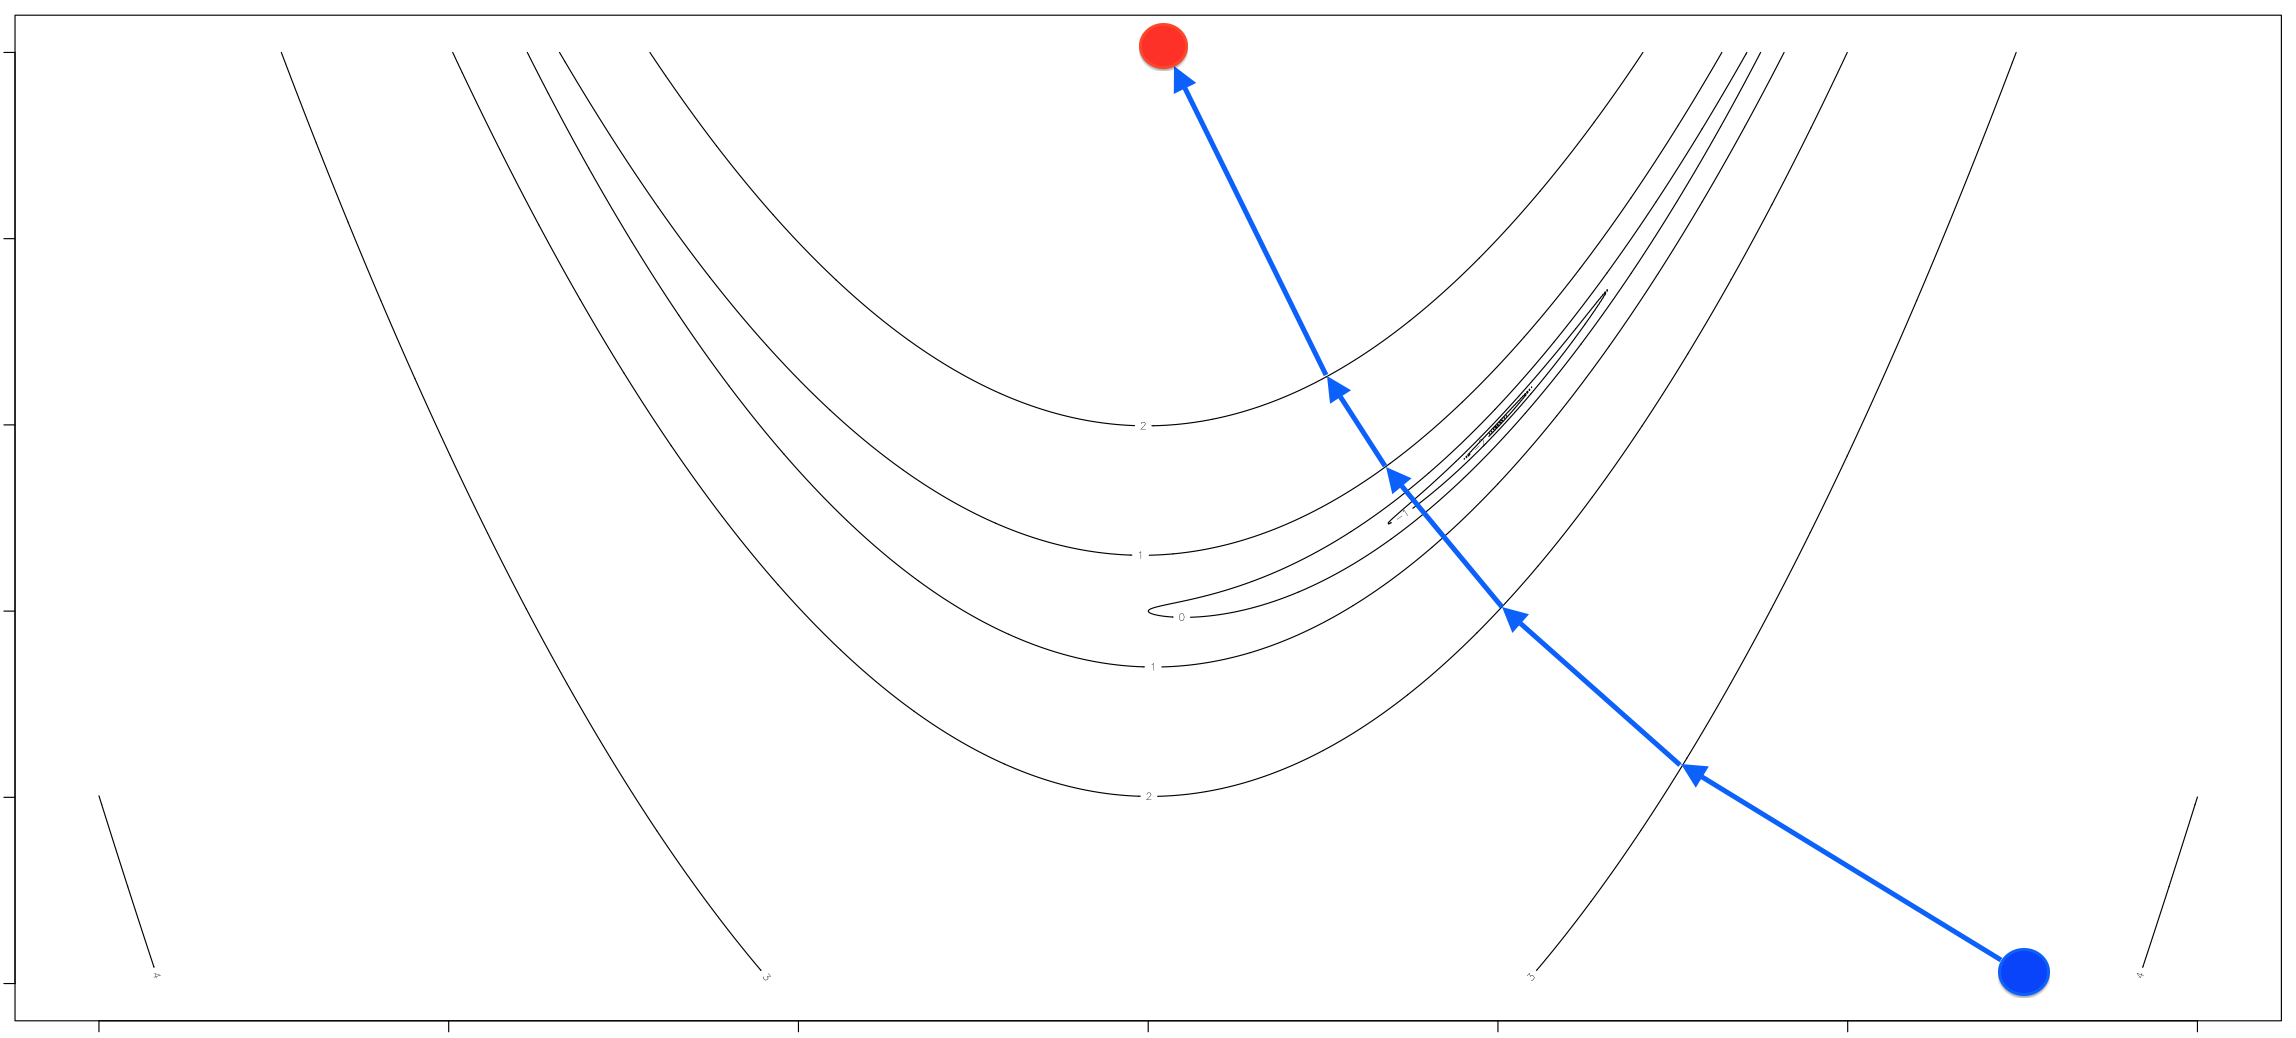
\includegraphics[width=16cm]{/Volumes/Mac OS Drive/Thesis/Source Code/Reporting/nwm_Report/images/gradient_descent_contour_plot.png}
\caption[The contour plot of a fictitious loss function]{\label{fig:contour_plot}A contour plot representing the surface of a simple \emph{fictitious} loss function. The approximation function follows the principle of steepest descent from its (blue) initiation point - crossing each contour line orthogonally - reaching the (red) global minimum at iteration number m$_{\text{stop}}$.}
\end{figure}

There are several weaknesses to this naive version of FGD, one of which is that any structural relationship between the approximation functions $\hat f_{(1)}^{[m_{stop}]} , … , \hat f_{(n)}^{[m_{stop}]}$ that act upon the data set are ignored. Simple relationships are assumed: $\hat f_{(1)}^{[m]} \rightarrow Y_i, … , \hat f_{(n)}^{[m]} \rightarrow Y_n$, which may fail to capture all the information held in the model variables. The algorithm defined in the following section addresses this weakness and improves further upon the progress this naive FGD method has made - describing the primary modelling tool used for this study.

\pagebreak


\subsection{Component-wise functional gradient descent \label{comp-boosting}}
\label{sec-1-4}


\subsubsection{Definition and properties \label{comp-alg}}
\label{sec-1-4-1}

With the two concepts of \emph{boosting} and \emph{gradient descent} having been defined, as well as the method of (batch) gradient boosting \cite{friedman2001greedy}, the final enhancement is to be introduced; defining \emph{component-wise} gradient boosting, which adds the last features that were outlined in Section \ref{gen-props}. Namely, that a form of variable selection be implemented\footnote{This is of great importance for this study, as the inclusion of lagged variables produces data sets where $p > n$.} within the boosting process. In addition to variable selection, as will be shown, this also inherently provides a certain amount of assurance of performance in the face of multicollinearity. Algorithm \eqref{alg-comp-boosting} defines the iterative procedure in which component-wise boosting minimises the empirical risk $\mathcal{R}$ (given in Equation \eqref{eqn-emp-risk}) over the approximation function, $f$.

\vspace{5mm}

\begin{algorithm}[H]
  \caption{Component-wise functional gradient boosting}
  \label{alg-comp-boosting}

  \BlankLine
  \BlankLine

  \SetKw{Return}{return} %% Custom keyword
  \KwIn{loss function, $\rho$; base-learners; counter, $m$; learning rate, $\nu \in [0,1)$}
  \KwOut{optimal prediction function: $f^*$}
  
  \BlankLine
  \BlankLine
  
  \begin{enumerate}[leftmargin=12.5mm]
  \item [Step 1.] Initialise the n-dimensional function estimate $\hat f^{[0]}$ with offset values\hspace{20pt} \texttt{/* e.g. $\coloneqq \mathbf{0}$ */}
  \item [Step 2.] Specify a set of $P$ base-learners; initialise the counter, $m \coloneqq 0$
  \item [Step 3.] Increase $m$ by one
  \item [Step 4.]
    \begin{enumerate}
    \item [a.] Compute the negative gradient of the loss function: $\mathbf{u}^{[m]} = - \frac{\partial \rho}{\partial f}$
    \item [b.] Evaluate the negative gradient at the previous iteration's model estimate
    \item [c.] Fit each of the $P$ base-learners to the resulting negative gradient
    \item [d.] Select the base-learner that best fits
      $\mathbf{u}^{[m]}$ by some criterion \hspace{35pt} \texttt{/* e.g. SSE */}
    \item [e.] Set $\mathbf{\hat u}^{[m]}$ equal to the best fitting base-learner
    \item [f.] Update current estimate $\hat f^{[m]} \coloneqq \hat
      f^{[m-1]} + \nu \cdot \mathbf{\hat u}^{[m]}$
    \end{enumerate}
  \end{enumerate}

  \Repeat{$m = m_{stop}$} {
    \BlankLine
    Steps 3 and 4
    \BlankLine
  }
  \BlankLine
  \BlankLine
  \Return{the prediction function that minimises $\rho$: $f^* = \hat f^{[m_{stop}]}$}
\end{algorithm}

\vspace{5mm}

\textbf{Step 1} sets the initial function estimate set to a zero-vector. The $P$ base-learners that are specified in \textbf{Step 2} are generally simple estimators that each take a pre-defined set of input variables and provide a univariate response. Each of them may take different subsets of the (entire) model's input variables; the subsets are usually relatively small, in order to make use of the model's features. The base-learners that are provided to a model for implementation within Algorithm \eqref{alg-comp-boosting} provide the tool that allows the modeller to stipulate structural assumptions regarding the model. Beyond simply grouping of variable subsets, several further options are available, such as methods to introduce categorical and ridge-penalised effects - refer to \cite{Hofner2012} for more information on these options.

In this study, the base-learners are least-squares estimators, with input of single predictor variables. Therefore, each base-learner fits a simple linear model against the negative gradient for each of the individual predictor variables. Coupled with shrinkage effects being applied to the best base-learner (due to $\nu < 1$ in \textbf{Step 4.f}), this individual predictor modelling highlights how component-wise gradient boosting is still able to perform, should there be relatively high levels of multicollinearity among the predictors. If the learning rate were selected to be $\nu = 1$, the resulting algorithm would be \emph{greedy} (just as the original AdaBoost algorithm) and so would not cope so well with multicollinearity. There is, however, an element of uncertainty in which predictor will be selected over the many iterations. If the correlation between two predictors is extremely high (e.g. $> 0.7$), which predictor is selected at each step may not be consistent - therefore it must be mentioned that there are limits to this facet of the variable selection feature of component-wise gradient boosting. This is taken into consideration within the empirical segment of this study, as discussed in Section \texttt{pairwise-corr}.

In \textbf{Step 4}, the computed negative gradient estimate is evaluated at the vector estimate of the previous iteration's approximation function, $\hat f^{[m-1]} \left( \mathbf{X}_{i}^\top \right)$, yielding Equation \eqref{eqn-neg-grad-vector}:

\begin{equation}
  \mathbf{u}^{[m]} = \left( u_{i}^{[m]} \right)_{i = 1, …, n} \coloneqq \left( - \frac{\partial}{\partial f}\rho\left(Y_i, \hat f^{[m-1]} \left( \mathbf{X_i^\top} \right) \right) \right)
  \label{eqn-neg-grad-vector}
\end{equation}

\vspace{3mm}

The criterion that is used for this study to select the best performing base-learner (as in Step \textbf{4.d.}) is the sum of squared errors (SSE), however this may be adapted to the model, for example in the case the base-learners should become more complicated and take forms other than linear models. $L_1$ absolute error might be a good alternative if the model should be more robust to outliers.
As a consequence of this study using base-learners containing only individual variables, the variable selection process (carried out in \textbf{Step 4.d.}) inherently extends to the notion of \emph{model selection}, in this particular case. As previously mentioned, the choice of base-leaner provides a means to specifying structural assumptions, and the efficacy of those choices can be seen in this step. The learning rate, $\nu$, for use in \textbf{Step 4.f.} should be a real number lying on the interval $\left[0 , 1 \right)$. More discussion on this parameter can be found in Section \ref{nu}. The last major point of interest within Algorithm \eqref{alg-comp-boosting} is the parameter $m_{stop}$. A method to approximate an optimal value for this important parameter is described in more detail in Section \ref{mstop}.

The model description given in Section \ref{comp-boosting} initialises the weights to zero. There are several reasons why this is a reasonable choice. Firstly, initialising the values to zero means that in the case of a particular variable never representing the closest approximation to the negative gradient of the loss function, $\mathbf{u}$ - by not once producing the base-learner fit with the lowest error over all variables - this variable is never selected and so its weight never incremented. Keeping in mind that these weights correspond to the coefficients of the variables in the final model, this then equates to the final value of this coefficient at completion of the gradient descent remaining untouched, equal to zero, ergo the variable is not selected for the final model. This is part of the intuition behind the inherent feature of variable selection presented by component-wise gradient boosting\footnote{Any possibility of a base-learner being incremented more than one time, and providing a final value $f_{i}^{[m_{stop}]}$ equal to zero, is completely ruled out by the requirement of the loss-function being convex. The increments for one particular base-learner (and so the variables contained) can only be of one sign, positive \textbf{or} negative, meaning the summation may never converge to zero. (Stochastic gradient boosting may, however, exhibit a non-zero possibility of this phenomenon.)}.
The second useful property of using zero as the initial weights is that, regardless of whether a coefficient evolves to be positive or negative at completion, the starting point was the same. To a moderate extent, this symmetry additionally facilitates the direct comparison of variable importance via their coefficients magnitudes, which tell us \emph{how far} each base-learner progressed the model along the surface of the loss function as it approached the minimum. This is of course a function of the negative gradient and the learning rate.

This section has summarised the main methodology used within this study; however some preliminary testing was also completed using several variants of this model. Some extra information explaining their usage is explained in the following sections.


\subsubsection{Parameter selection \label{param-selection}}
\label{sec-1-4-2}


\paragraph{Learning rate: $\nu$ \label{nu}}
\label{sec-1-4-2-1}

The learning rate, $\nu$, is commonly held constant throughout the boosting process, which has proven to be a simple, yet effective method. To see why this approach is indeed an elegant, we must inspect the magnitude of the increments to our approximation function during the gradient descent, not only the scalar learning rate itself. One might consider different learning rates and their effect on the speed of approach to the loss-function's minimum (given there being only one global minimum). Given a tiny learning rate, the speed of approach would be extremely slow; however, offering a very close approximation to the minimum as a by-product. Selecting a large learning rate would conversely allow for a rapid descent towards the minimum; however, offering relatively little precision. The truth, however, is that the increments that are added to our approximation function at each iteration \emph{are} indeed adaptive - in terms of the negative gradient, which must decrease as the gradient descent approaches the minimum, by the definition of the loss function being convex. This can be seen in Figure \ref{fig:grad-descent}, where a simple one-dimensional case is demonstrated.

\begin{figure}[htb]
\centering
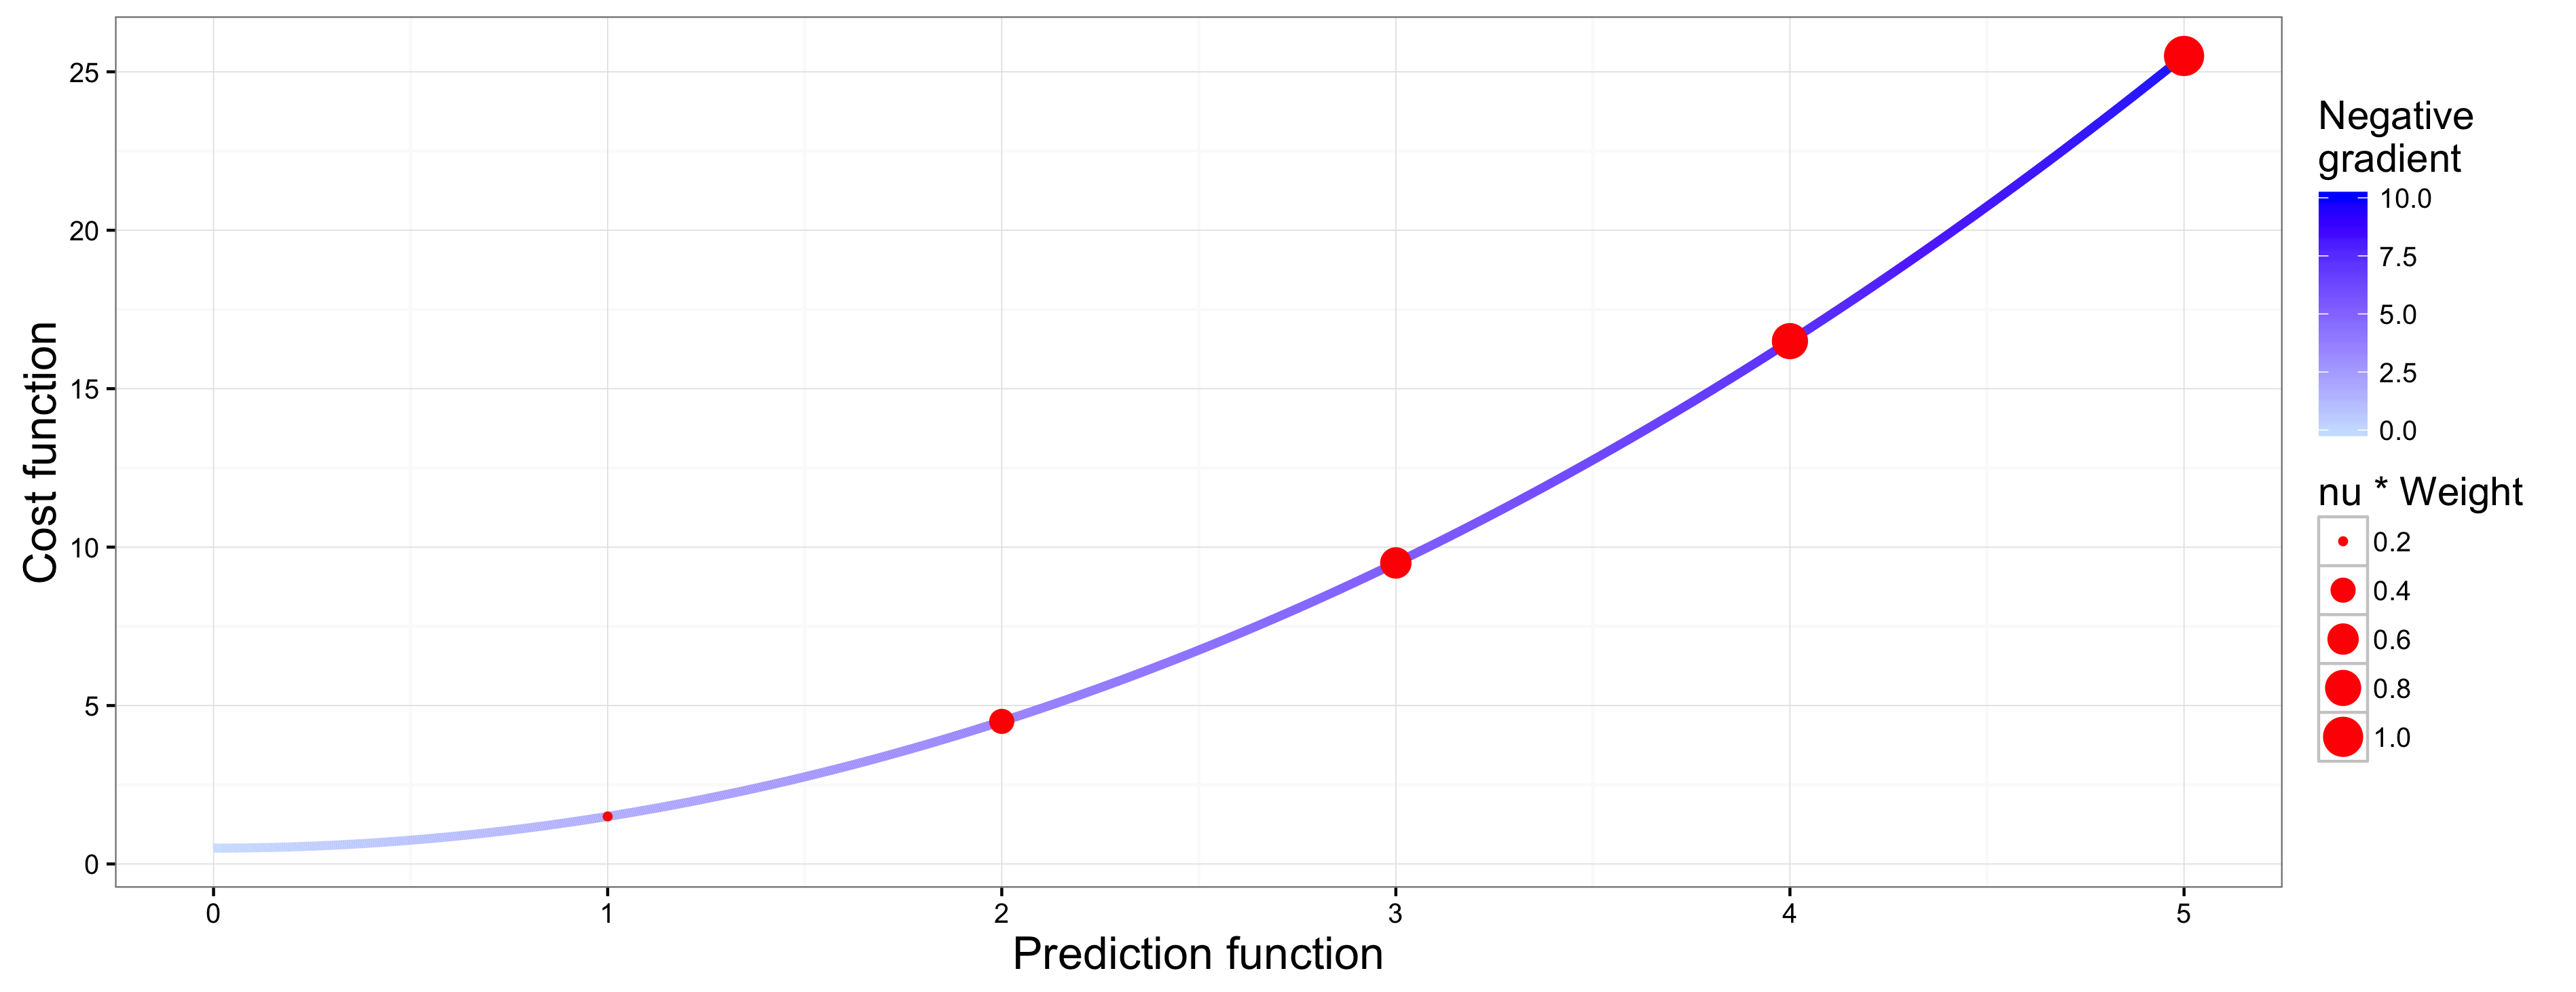
\includegraphics[width=16cm]{/Volumes/Mac OS Drive/Thesis/Source Code/Reporting/nwm_Report/images/learning_rate-neg_gradient.png}
\caption[An example loss function for the one-dimensional case]{\label{fig:grad-descent}A loss function for the one-dimensional case; the size of the red points along the curve representing the incremental addition to approximation (prediction) function during gradient descent. Holding $\nu$ constant, it is clear that the nominal step-size, $\nu \cdot \left( - \frac{\partial}{\partial f}\rho (Y, f)\right)$, does indeed adapt in size at each iteration.}
\end{figure}

A fictitious loss function is plotted for the one-dimensional case (the parabola: $y = x^2 + \frac{1}{2}$), where the colour gradient of the curve reflects the magnitude of the negative gradient, $u = \left( - \frac{\partial}{\partial f}\rho (Y, f)\right)$; dark blue indicates a steep gradient, which slowly lightens as the function levels out to its minimum. A value for $\nu$ of $0.1$ is defined, giving the size of the red points reflects the magnitude, $\nu \cdot u$, by which the approximation function is incremented during gradient descent. It is clear that the gradient descent will take steps of ever decreasing length as the minimum is approached, the decrease in step-site proportional to the reduction in the gradient. Therefore there is no obvious benefit gained by e.g. adaptively decreasing $\nu$ over the iteration process. The accuracy this method offers, via the self-adapting step-length, is assumed to provide sufficient precision when approximating the loss function's minimum, even though $\nu$ is held constant.

Of course the \emph{constant} value of $\nu$ is still a model parameter to be optimised, if not for precise approximations, for the the gradient descent to be performed as efficiently as possible in terms of computational cost. For performance, it is shown by the authors \cite{schmid2008boosting} to suffice to use a small value, e.g. $0.1$, as is demonstrated in Figure \ref{fig:grad-descent}. It must lie on the half-open interval $\left(0 , 1 \right]$, The usage of this variable within this study is discussed within Section \texttt{param-grid}. Furthermore, to dynamically adapt the step-size factor to the iteration count of the negative gradient does not improve the estimates of $f^*$, and will only increase the computational cost of running a descent to convergence. It is worth noting, additionally, that large values may prevent convergence to the minimum, and could even lead to cases of divergence\footnote{To show this, one must simply use the argument presented in Figure \ref{fig:grad-descent}, instead using a large value of $\nu$ to see that the minimum may easily be overshot.}.


\paragraph{Stopping iteration: $m_{stop}$ \label{mstop}}
\label{sec-1-4-2-2}

As already discussed in previous sections, there are two main input parameters that have a large effect on the overall performance of the boosting algorithm: $\nu$ and $m_{stop}$. The learning rate, $\nu$, must be assigned a sensible value (which depends upon the input data); however, has the lesser impact of the two parameters. The more important model parameter is the number of boosting iterations, i.e. when to end the gradient descent algorithm, which requires optimisation with regards to the data set at hand. Up until this point, this was merely labelled as the point when Algorithm \eqref{alg-comp-boosting} converges, $m_{stop}$; in practice however, the exact value is less well defined and must be optimised empirically. One must consider the reality of \emph{overfitting} the model to the in-sample (\emph{training}) data set. If the model trains too closely to the data, the resulting prediction function will likely perform badly in out-of-sample testing. It is therefore necessary to perform some manner of cross validation on the results obtained from the gradient descent procedure.

One could perform the cross-validation in a number of ways, for example, using (1) k-fold cross validation, (2) sub-sampling and (3) bootstrapping methods - all of which are implemented within the \texttt{mboost} package, via the function: \texttt{cvrisk()}. This study exclusively made use of bootstrapping methods, whereby the number of cross-validation replications used was 25. The output model objects (created by the \texttt{mboost\_fit} function) do not simply contain the final approximation function with the coefficients of the selected variables, but rather the information from every iteration from the gradient descent. The cross-validation can then bootstrap the results at each boosting iteration and record the error. Executing 25 bootstrapped replications then allows the average (squared) error to be computed - the iteration that holds the minimum value from this set of results indicates the optimal value of iterations, $m_{stop}$. 

Consider a model that was produced from component-wise boosting, running in total for 100 iterations. Figure \ref{fig:cvrisk-example} illustrates the cross-validation methodology on the outcome, illustrating how the optimal number of iterations, $m_{stop}$, is identified. The iteration number is selected, where the minimum error over the 25-bootstrapped samples is found - the process is labelled an \emph{early stopping strategy}, which aims to optimise the final models prediction accuracy.

\begin{wrapfigure}{l}{0.5\textwidth}
\centering
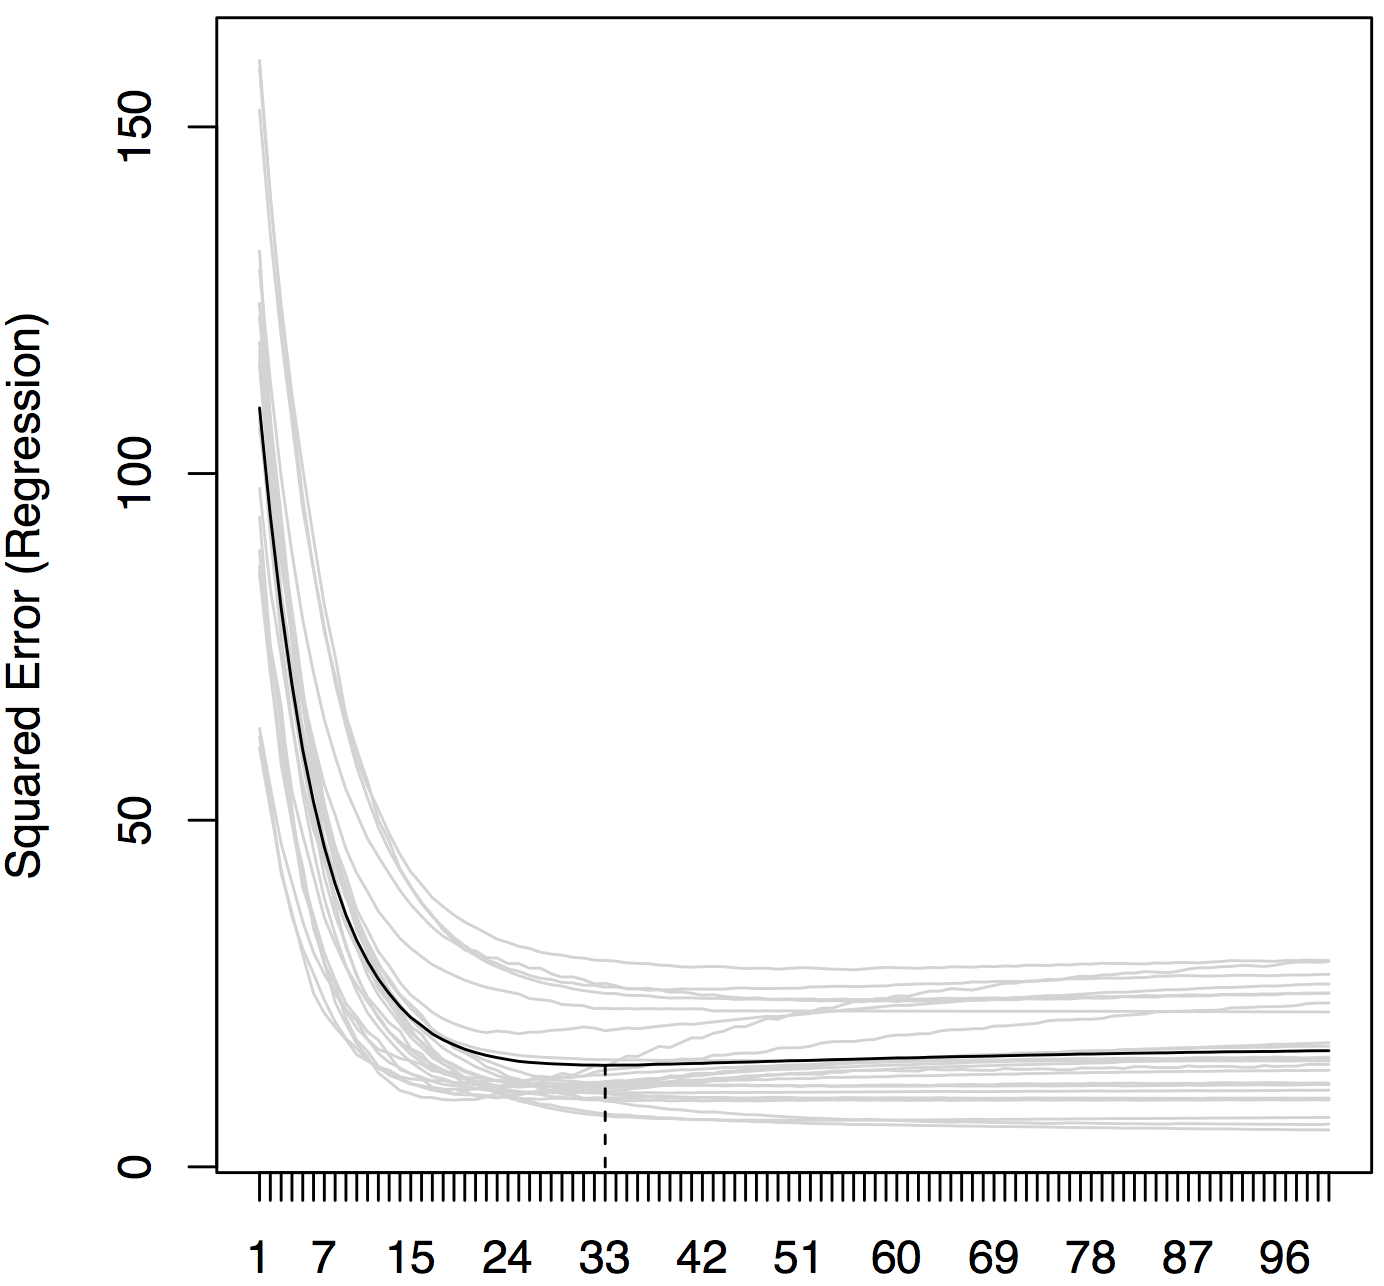
\includegraphics[width=0.48\textwidth]{/Volumes/Mac OS Drive/Thesis/Source Code/Reporting/nwm_Report/images/cvrisk-example.png}
\caption[An illustration of 25-fold boostrap cross-validation]{\label{fig:cvrisk-example}Example of 25-fold bootstrap cross-validation for a model with 100 iterations. Each of the 25 light grey lines shows the error at each iteration for each bootstrap. The black line displays the average over all bootstrap results. The minimum of the averaged error is highlighted with a dashed vertical line m$_{\text{stop}}$ = 33. Source: \cite{Hofner2012}.}
\end{wrapfigure}

The $m_{stop}$ parameter affects the level of relative complexity\footnote{The term 'complexity' is naturally somewhat subjective, being model dependent.} that the chosen model exhibits. If the final approximation function is selected, which was produced at the hundredth iteration (in the example given), the model is likely to include many parameters, which were selected in an exhaustive search for the minimum of the loss function. Parameters that perhaps have little effect on the outcome variable may have been included, leading to overfitting. In comparison, the value of m$_{\text{stop}}$ obtained from (bootstrap) cross-validation not only has a lower average squared error (by definition), but is also likely to return much simpler model. Less iterations would have been performed, meaning that less variables in a wide data set can have been selected, and those that were selected are the influential variables. As can be seen from Figure \ref{fig:cvrisk-example}, the error reaches a minimum quit early on, and plateaus out. This means the approximation function at iteration $m_{stop} = 33$ explains just as much variance in the data set as the model at iteration $m = 100$, so selecting the simpler model is good practice (by arguments of model parsimony, i.e. 'Ockham's Razor').

The \texttt{mboost} literature, \cite{Hofner2012}, also discusses usage of alternative criteria in order to locate the $m_{stop}$ value. The example given is that of the Akaike Information Criterion (AIC). It is suggested that this method, however, tends to produce larger values of $m_{stop}$, which overshoot the minimised squared error shown through cross-validation.


\subsection{Stochastic gradient boosting \label{stochastic-boosting}}
\label{sec-1-5}

The introduction of a stochastic component to gradient boosting has proved to be a great tool in reducing the standard errors in a final prediction model by variance reduction, especially when the predictors show signs of correlation. The idea of variance reduction is already seen in older machine learning algorithms such as \emph{bagging} (bootstrap aggregation) and random forests \cite{breiman2001random}. The former creates many subsets of the training data to fit many models, and taking the average produces results with smaller errors than would've been found by using the whole training data. The bootstrapping procedure is out-of-bag (OOB) with replacement, meaning some variables will be selected many times and other perhaps not at all, depending on the setup. Random forests enhances bagging further still by saying (in terms of classification trees): at each stage when a tree has been fitted to one of the bootstrapped samples, select a subsets $m$ of the $p$ variables from the terminal nodes \textbf{\emph{at random}}, then select only the best variable among those $m$ variables for the next split point.

This insertion of a stochastic procedure - randomly selecting from the variables after fitting the tree - squeezes as much variance reduction as possible into the modelling and therefore reduces the final error as much as possible when averaging. It is this notion that is applied to gradient boosting, thus making it stochastic. The random selection can occur at one of two places, creating either a random subsets of the training data (à la bagging), or a random subset of the features found at each step (à la random forests). The randomness in the model fit and reduction in final estimate errors, coupled with a slower loss-function descent, may also hinder over-fitting and so improve the models ability to generalise to out-of-sample data.

Other than the inclusion of this simple step into the method that was set out in Section \ref{grad-boosting}, no other changes are made to the iterative procedure. As one may expect, removing information at each iteration can mean that some of the other model hyper-parameters must be adjusted, i.e. differing optimal values are likely to be found. The tendency is for the model to require a larger number of iterations to descend along the surface of loss function to the minimum.

Additionally, of course, there is the introduction of a new hyper-parameter, namely the proportion of data or features that are to be selected at random. This parameters can also be optimised for; however, Friedman (\cite{friedmanstochastic} Page 5, Figure 1) found that values between 50 \% and 80 \% provided the lowest errors.

A small practical note: the R package \texttt{mboost} has the functionality of the bagging approach, sub-sampling the input data, but does not support the random forest enhancement. The functionality is, however, provided by the \texttt{gbm} package, which finds implementation within this study, in Section \ref{stochastic-boosting}.


\subsection{Families of distributions}
\label{sec-1-6}

Depending on the requirements of the model, a specific family must be selected. The \texttt{mboost} package in R supplies many families. They are listed, along with their properties in Table 4 of \emph{Model-based Boosting in R} \cite{Hofner2012}. This section briefly outlines the practical aspects of several further families of regressors that are used within this study. A rudimentary outline is provided to explain in which situation each family may be used, indicating why the methods were required in several aspects of the empirical work.


\subsubsection{Gaussian}
\label{sec-1-6-1}

This family was used extensively for the general linear models performed on all data sets in order to predict stock market movements, discussed further in Section \texttt{main-modelling}. The Gaussian family is used in order to provide the conditional mean of a continuous response. In this case, the assumption is that the conditional outcome distribution, $\mathbf{Y}|\mathbf{X}$, is normally distributed and that the loss function is the negative Gaussian log-likelihood, which is equivalent to the $L_2$ loss - given in Equation \eqref{eqn-sqaured-error}:

\begin{equation}
  \rho (Y, f(X)) = \frac{1}{2} \cdot (Y - f(X))^2
  \label{eqn-sqaured-error}
\end{equation}


\subsubsection{Binomial}
\label{sec-1-6-2}

This family is used in order to model a binomial \emph{class} response\footnote{As a practical note, the \texttt{Binomial()} family within the \texttt{mboost} package returns values \{-1, 1\} in its binary response, for reasons of computational efficiency.}: \{0, 1\}. Just as the Gaussian family, the binomial family was used on all data sets in this study to predict the direction of the market, but without regard for the magnitude. Analogously to the Gaussian family, the probability parameters may be approximated through the minimisation of the negative \emph{binomial} log-likelihood - given in Equation \eqref{eqn-bin-error}:

\begin{equation}
  \label{eqn-bin-error}
  \rho (Y, f(X)) = - \left[ Y \cdot log(\mathbb{P} (Y = 1 \mid X)) + (1-Y) \cdot log(1 - \mathbb{P} (Y = 1 \mid X)) \right]
\end{equation}



\subsubsection{Gamma}
\label{sec-1-6-3}

This family allows predictions to be made purely of the magnitude of stock market movements, with no regard for the direction. The gamma distribution, implemented as the \texttt{GammaReg} family within the \texttt{mboost} package, and provides a continuous non-negative response, required for such a model. This function uses the negative gamma-likelihood coupled with the logarithmic link function. For more information on this distribution and estimates of its parameters, refer to \cite{Hofner2012} and \cite{choi1969maximum}.


\subsubsection{Inspection within R}
\label{sec-1-6-4}

Listing \ref{code:family} illustrates how one may inspect a family contained within the \texttt{mboost} package, directly within the R console. On line 1 the \texttt{mboost} package is first loaded into the session. The details of the Gaussian family are called up on line 3 and the information about the negative gradient on line 10. Similar operations may be performed for many of the families that the \texttt{mboost} package contains.

\vspace{5mm}

\begin{listing}[H]
\begin{minted}[frame=lines,linenos]{r}
  R > library(mboost)

  R > Gaussian()

        Squared Error (Regression) 

        Loss function: (y - f)^2 


  R > slot(Gaussian(), "ngradient")

        function (y, f, w = 1) 
    
        y - f
\end{minted}
\caption[A guideline to inspecting the \texttt{mboost} Gaussian family]{\label{code:family}An example of how to investigate the properties of an implemented \emph{family} within the \texttt{mboost} package - here the example of the Gaussian family.}
\end{listing}
% Emacs 24.5.1 (Org mode 8.2.10)
\end{document}